\documentclass[a4paper,14pt]{extarticle}
\usepackage{../../tex-shared/report-layout}

\renewcommand{\mylabnumber}{1}
\renewcommand{\mylabtitle}{Исследование возможностей языка
R для статического анализа данных}
\renewcommand{\mysubject}{Интеллектуальный анализ данных}
\renewcommand{\mylecturer}{Сырых О.А.}

\begin{document}
\begin{titlepage}
    
    \thispagestyle{empty}
    
    \begin{center}
        
        Министерство науки и Высшего образования Российской Федерации \\
        Севастопольский государственный университет \\
        Кафедра ИС
        
        \vfill

        Отчет \\
        по лабораторной работе №\mylabnumber \\
        \enquote{\mylabtitle} \\
        по дисциплине \\
        \enquote{\MakeTextUppercase{\mysubject}}

    \end{center}

    \vspace{1cm}

    \noindent\hspace{7.5cm} Выполнил студент группы ИС/б-17-2-о \\
    \null\hspace{7.5cm} Горбенко К. Н. \\
    \null\hspace{7.5cm} Проверил \\
    \null\hspace{7.5cm} \mylecturer

    \vfill

    \begin{center}
        Севастополь \\
        \the\year{}
    \end{center}

\end{titlepage}

\section{Цель работы}
\begin{itemize}
    \item изучить основные особенности языка R;
    \item исследовать возможности языка R для работы с графикой.
\end{itemize}

\section{Задание на работу}
\begin{enumerate}
    \item Установить R на ПК.
    \item Установить RStudio - инсталлятор скачать с официального сайта проекта.
    \item Ознакомиться с кратким руководством пользователя RStudio.
    \item Исследовать команду \code{\enquote{demo()}}, полученные результаты вставить в отчет.
    \item Исследовать основные функции и команды языка R, представленные в данной
          лабораторной работе, полученные результаты вставить в отчет.
    \item Ответить на контрольные вопросы.
\end{enumerate}

\section{Ход работы}
Используем консоль \code{R.exe}. При входе получаем следующий текст:

\begin{lstlisting}
R version 3.6.2 (2019-12-12) -- "Dark and Stormy 
Copyright (C) 2019 The R Foundation for Statistic
Platform: x86_64-w64-mingw32/x64 (64-bit)

R is free software and comes with ABSOLUTELY NO W
You are welcome to redistribute it under certain 
Type 'license()' or 'licence()' for distribution 

    Natural language support but running in an Engl
'citation()' on how to cite R or R packages in publications.

Type 'demo()' for some demos, 'help()' for on-line help, or
'help.start()' for an HTML browser interface to help.
Type 'q()' to quit R.
\end{lstlisting}

Выполним команду \code{demo()}. Результат выполнения команды представлен
на рисунке \ref{fig:demo}.
\begin{figure}[H]
    \centering
    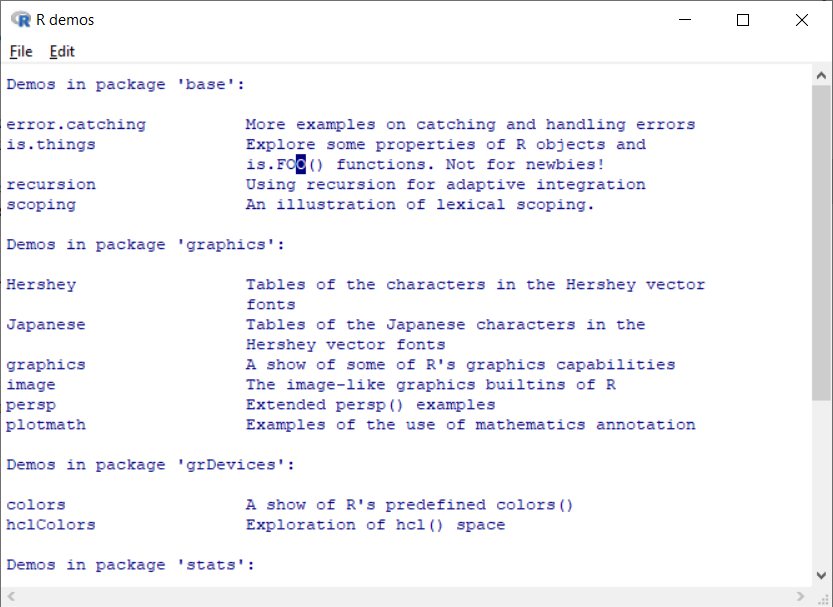
\includegraphics[width=.8\linewidth]{demo}
    \caption{Результат выполнения команды \code{demo()}}
    \label{fig:demo}
\end{figure}

Выполним команду \code{help(demo)}. Результат ее выполнения изображен на рисунке \ref{fig:help-demo}
\begin{figure}[H]
    \centering
    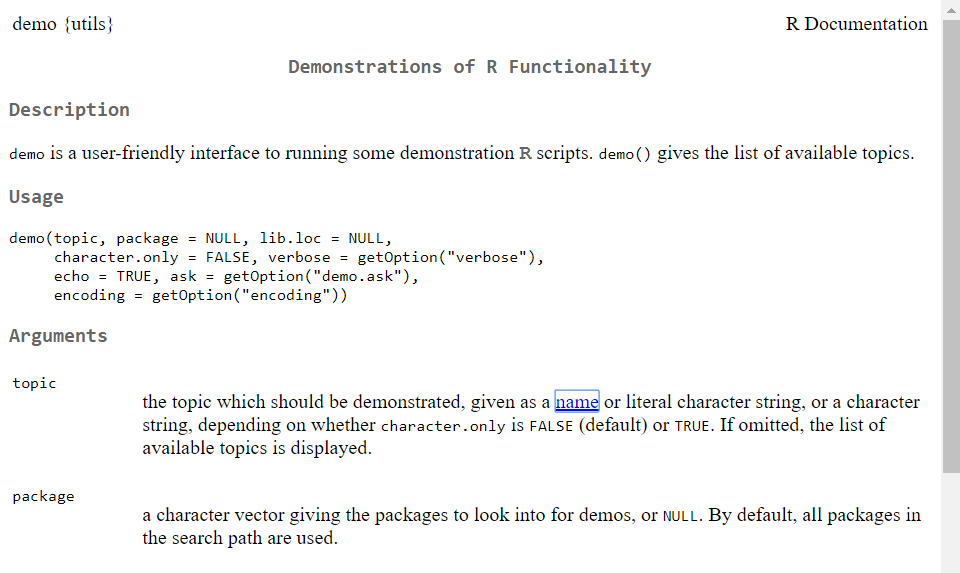
\includegraphics[width=.8\linewidth]{help-demo}
    \caption{Результат выполнения команды \code{help(demo)}}
    \label{fig:help-demo}
\end{figure}

Работа с векторами:
\begin{itemize}
    \item c() – создать вектор небольшой длины;
    \item scan() – считывание последовательно вводимые с клавиатуры значения;
    \item mean() – вычисляет среднее значение элементов вектора;
    \item paste() –  объединяет элементы множества текстовых векторов;
    \item sort() – сортировка элементов вектора по возрастанию или убыванию;
    \item class() – проверка типа вектора;
    \item sd() – стандартное отклонение.
\end{itemize}
\begin{lstlisting}
> v1 <- c(1, 2, 3, 4, 5) * 3
> v1
[1]  3  6  9 12 15
> v1[1:3]
[1] 3 6 9
> v2 = rep(15, 4)
> v2
[1] 15 15 15 15
> length(v2)
[1] 4
\end{lstlisting}

Работа с матрицами:
\begin{itemize}
    \item \%*\% – матричное умножение;
    \item t(x) – транспонировать матрицу;
    \item diag(x) – диагональ матрицы;
    \item solve(a, b) – решает систему уравнений;
    \item solve(a) – обратная матрица;
    \item colSums, rowSums, colMeans, rowMeans – сумма и средние по столбцам и строкам.
\end{itemize}
\begin{lstlisting}
> mat1 <- matrix (data=1, nrow=3, ncol=3)
> mat1
    [,1] [,2] [,3]
[1,]    1    1    1
[2,]    1    1    1
[3,]    1    1    1
> is.matrix(mat1)
[1] TRUE
> dim(mat1)
[1] 3 3
> dim(mat1)
[1] 3 3
\end{lstlisting}

Работа с графикой:
\begin{itemize}
    \item matplot(x,y) – график зависимости столбцов y от столбцов x;
    \item foutfoldplot(x) – изображает (в виде частей окружности) связь между
          двумя бинарными переменными в разных совокупностях;
    \item assocplot(x) – график Кохена-Френдли;
    \item pairs(x) – функция изображает диаграммы рассеяния для всех возможных
          пар переменных из матрицы x;
    \item plot.ts(x), ts.plot(x) – изображает временной ряд;
    \item qqnorm(x) – квантили;
    \item qqplot(x, y) – график зависимости квантилей y от квантилей x;
    \item contour(x, y, z) – выполняет интерполяцию данных и создает контурный
          график;
    \item symbols(x, y) – изображает различные символы в соответствии с
          координатами;
    \item termplot(mod.obj) – изображает частные эффекты переменных из
          регрессионной модели;
\end{itemize}

\begin{lstlisting}
> x <- c(1, 2, 3, 4, 5)
> y <- c(1, 2, 3, 4, 5)
> plot(x, y, type="l")
> plot(atan, -2 * pi, 2* pi)
\end{lstlisting}

Результат выполнения программы:
\begin{figure}[H]
    \centering
    \subfloat[y = x]{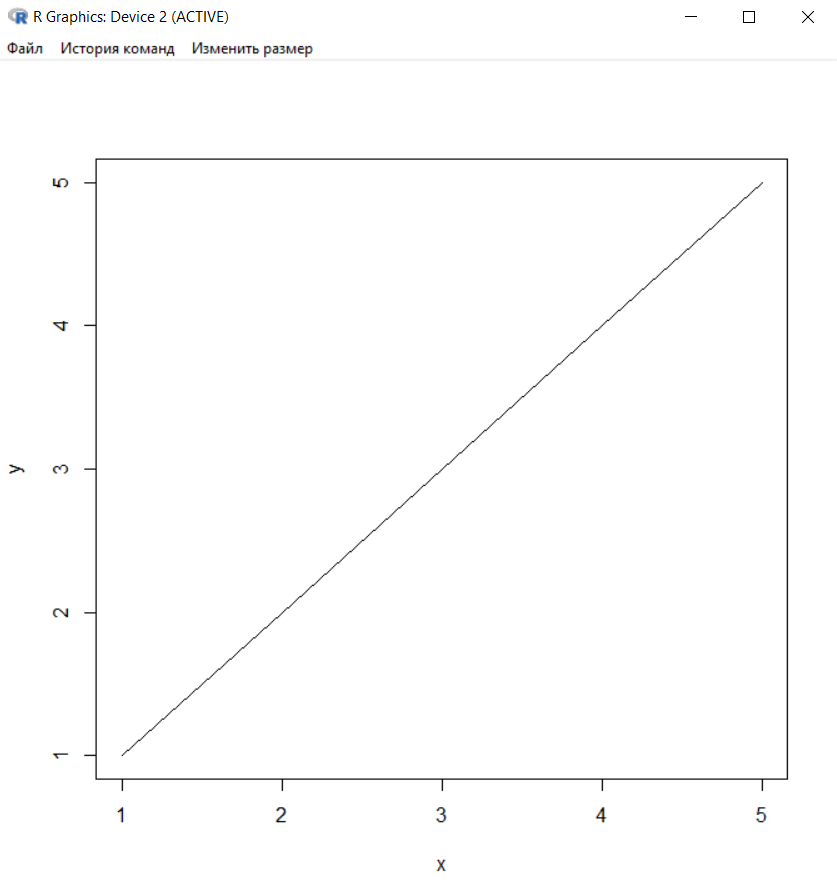
\includegraphics[width=.4\linewidth]{y=x}}
    \hspace{.15\linewidth}
    \subfloat[y = arctan(x)]{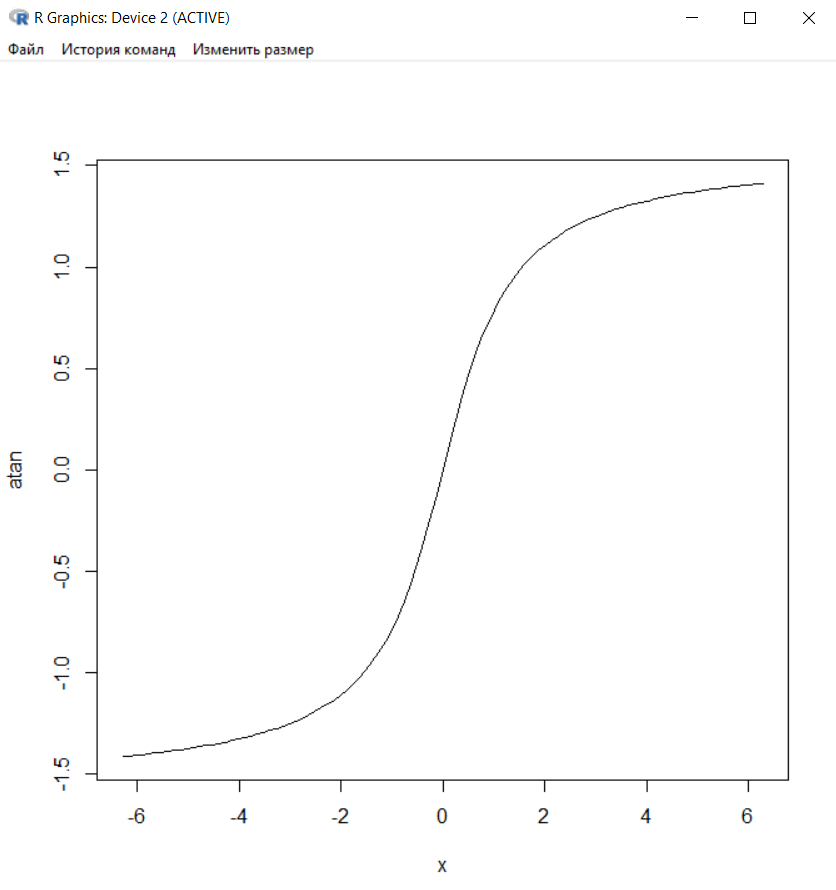
\includegraphics[width=.4\linewidth]{atan}}
    \caption{Демонстация работы с графикой}
\end{figure}

\section{Контрольные вопросы}

\subsection{Особенности языка R}
Язык R  — язык программирования для статистической обработки данных и работы
с графикой, а также свободная программная среда вычислений с открытым
исходным кодом.

R — интерпретируемый язык программирования, основным способом работы с
которым является командный интерпретатор. Язык объектный: любой программный
объект в нём имеет набор атрибутов — именованный список значений,
определяющих его.

Язык поддерживает минимальный набор примитивных типов данных: символьный,
числовой, логический и комплексный. Числовые переменные, помимо обычных
чисел, могут принимать специальные значения NaN (Not a Number — «не число»)
и Inf (Infinity — «бесконечность»). Бесконечность (положительная или
отрицательная) получается при выходе результата вычислений за пределы
представимого реализацией диапазона, NaN — при операциях с неопределённым
результатом. Помимо этих, имеется ещё одно очень важное специальное
значение, NA (Not Available — «не доступно»). Оно может быть использовано
для фиксации того факта, что соответствующее значение, участвующее в
вычислениях, по какой-либо причине не было.

Значения примитивных типов могут объединяться в векторы (vector), списки
(list), матрицы или массивы (matrix), в том числе многомерные; эти
комбинированные типы хранят наборы данных одного и того же примитивного
типа. Помимо этого, язык содержит понятие факторов (factor) — наборов
категориальных или шкальных данных, принимающих строго определённый набор
значений. Наконец, могут создаваться таблицы (data frame) — структуры
данных, которые для каждой строки (индивида) хранят набор различных (и
имеющих разные типы) параметров (признаков). Особенностью R является то, что
операции с векторами и матрицами поддерживаются на уровне самого языка.

Существует операция извлечения и записи данных (аналог присваивания) “<-“, а
также обычные операции работы с данными, в том числе арифметические. Доступ
по индексу к элементам векторов и массивов осуществляется с помощью
квадратных скобок (отсчет производится с 1), доступ к атрибутам списков —
посредством оператора «\$». Имеется минимальный набор обычных конструкций
императивного программирования: условный оператор if, циклы while и for.
Выражения на R можно описывать как отдельные объекты и вычислять по мере
необходимости. На этом же механизме основано описание функций.

Функции R могут объединяться в пакеты — загружаемые модули, которые
подключаются к любой программе и предоставляют объединённые в них
вычислительные средства. Пакеты для R могут разрабатываться на других языках
программирования, в том числе на Си.

Сам язык имеет довольно ограниченные и не слишком удобные средства описания
данных, но это компенсируется наличием библиотечных средств, которые
позволяют загружать в виде таблиц R наборы данных, представленных в
большинстве открытых и многих проприетарных форматах. Так, в R могут быть
легко загружены таблицы в простом текстовом формате, таблицы Excel различных
версий, данные в форматах CSV, XML и многих других.

В R реализованы практически все актуальные средства универсальных
статистических вычислений, такие как регрессионный анализ и анализ временных
рядов, а также множество специфических алгоритмов для решения
узкоспециализированных задач и исследований в отдельных областях.

\subsection{Команда для получения подробной информации о функции в R}
Для получения подробной информации (справки) о любой функции, необходимо
выполнить команду: \\ \code{help(имяФункции)} (\code{?имяФункции}).

\subsection{Структура и особенности команды \code{round()} в R} \code{round(x,
digits = 0)} - функция для округления значения(значений) первого параметра до
количества символов после запятой, задаваемого вторым параметром (0 по умолчанию).

Из-за различной реализации стандарта IEEE 754 на разных системах поведение
\code{round()} при округлении символа 5 может отличаться (округляет в большую
либо меньшую сторону)

Отрицательный параметр количества символов обозначает округление до степени 10.

\subsection{Команды для работы с векторами в R}
\begin{itemize}
    \item c() – создать вектор небольшой длины;
    \item scan() – считывание последовательно вводимые с клавиатуры значения;
    \item mean() – вычисляет среднее значение элементов вектора;
    \item paste() –  объединяет элементы множества текстовых векторов;
    \item sort() – сортировка элементов вектора по возрастанию или убыванию;
    \item class() – проверка типа вектора;
    \item sd() – стандартное отклонение.
\end{itemize}

\subsection{Команды для работы с матрицами в R}
\begin{itemize}
    \item \%*\% – матричное умножение;
    \item t(x) – транспонировать матрицу;
    \item diag(x) – диагональ матрицы;
    \item solve(a, b) – решает систему уравнений;
    \item solve(a) – обратная матрица;
    \item colSums, rowSums, colMeans, rowMeans – сумма и средние по столбцам и строкам.
\end{itemize}

\subsection{Работа с графикой в R}
\begin{itemize}
    \item matplot(x,y) – график зависимости столбцов y от столбцов x;
    \item foutfoldplot(x) – изображает (в виде частей окружности) связь между
          двумя бинарными переменными в разных совокупностях;
    \item assocplot(x) – график Кохена-Френдли;
    \item pairs(x) – функция изображает диаграммы рассеяния для всех возможных
          пар переменных из матрицы x;
    \item plot.ts(x), ts.plot(x) – изображает временной ряд;
    \item qqnorm(x) – квантили;
    \item qqplot(x, y) – график зависимости квантилей y от квантилей x;
    \item contour(x, y, z) – выполняет интерполяцию данных и создает контурный
          график;
    \item symbols(x, y) – изображает различные символы в соответствии с
          координатами;
    \item termplot(mod.obj) – изображает частные эффекты переменных из
          регрессионной модели;
\end{itemize}

\section*{Выводы}
В ходе лабораторной работы было получено начальное представлене об особенностях
языка (платформы R): о запуске интерпретатора, об операторах, об операциях над
векторами, матрицами, о работе с графикой.

\end{document}